
\section{External World Interfaces}
\subsection{General Purpose Input-Output Ports (GPIO)}
\subsubsection{General Characteristics of I/O Ports}
\begin{itemize}
    \item Allow comunication with the external world
    \item Operate digitally and can be configured as either inputs or outputs
    \item Can be configured individually or in groups called ports
\end{itemize}
\begin{multicols}{2}
    \subsubsection{Structure of an Input-Output Pin}
    \begin{itemize}
        \item Input Pins
        \item Output Pins
        \item GPIO Interfaces
        \subitem Allow configuring the oerpation of a particular pin as either IN or OUT  
    \end{itemize}
    
    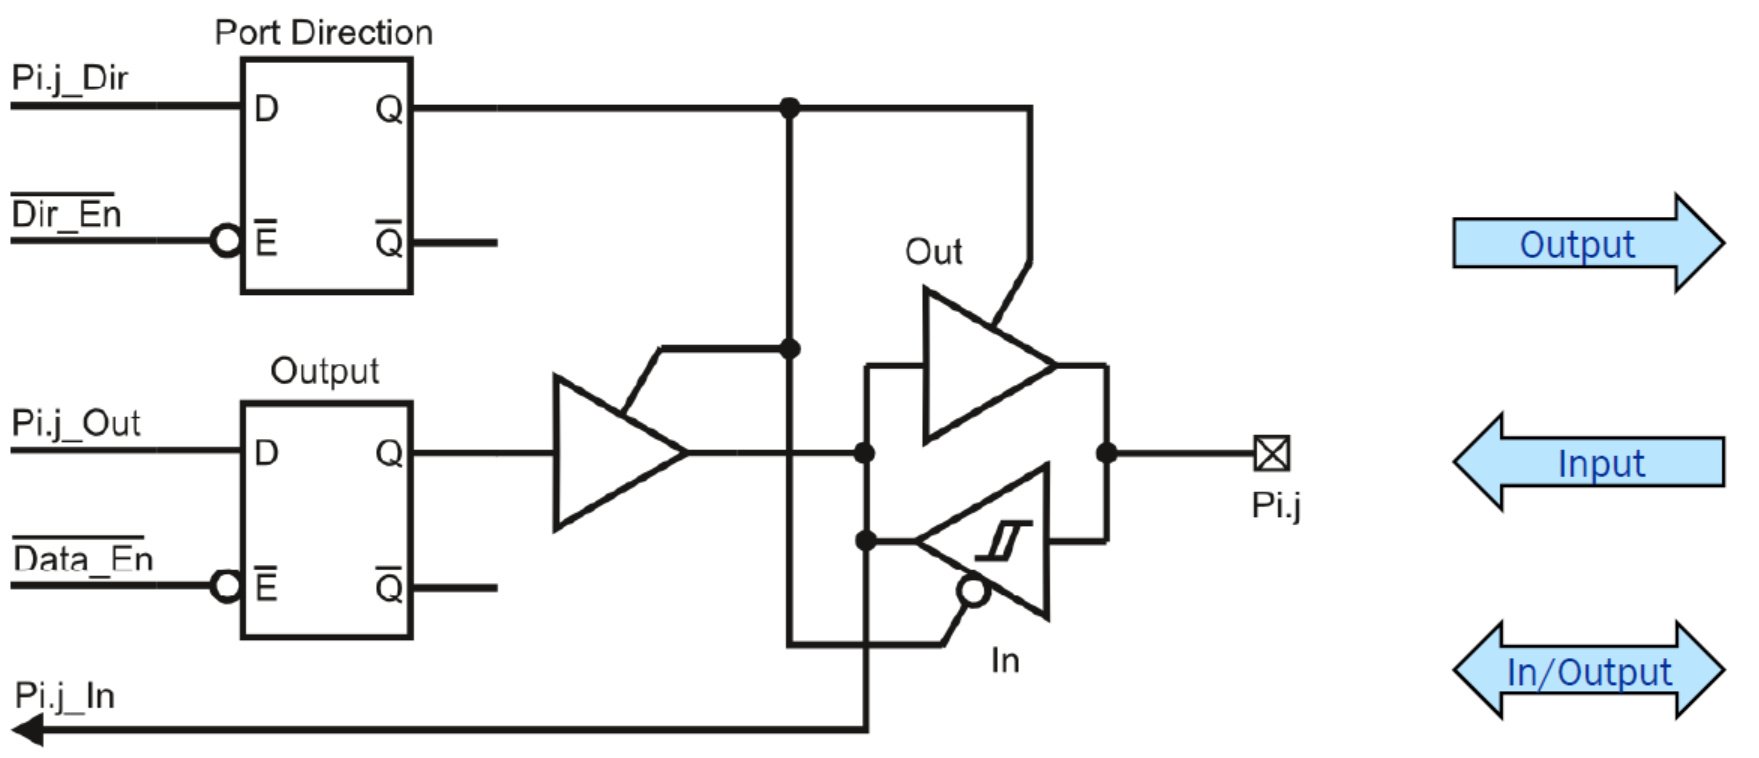
\includegraphics[width=\linewidth]{images/IOStructure}  
\end{multicols}

\subsubsection{MSP430 GPIO Registers}
\begin{tabular}{lll}
    PxSEL   &Port x Function Select             & Sets pin functionality  \\ 
    PxDIR   &Port x Data Direction              & Sets pin as either IN or OUT \\ 
    PxOut   &Port x Out                         & Data-out register \\ 
    PxIN    &Port x Input                       & Data-in register  \\ 
    PxIFG   &Port x Interrupt Flag              & Interrupt request for port x \\ 
    PxIES   &Port x Interrupt Edge Selection    & Sets signal edge to trigge interrupts in Port x input  \\ 
    PxIE    &Port x Interrupt Enable            & Enables interrupts from Port x pins \\ 
    PxREN   &Port x Ressistor Enable            & Enables internal pull-up/down resistors \\ 
    PxDS    &Port x Drive Strength              & Sets driver strength for port pins to up to 30mA  \\ 
    PxIV    &Port x Interrupt Vector            & Priority encoding for port Interrupts \\ 
\end{tabular} 


%TODO Chapter 08 ab seite 10
\clearpage